\documentclass[12pt]{article}
\usepackage[margin=1in]{geometry}
\usepackage{graphicx}
\usepackage{booktabs}
\usepackage{amsmath}
\title{The Effect of Paid Search Advertising on Revenue: \\
A Replication of the eBay Natural Experiment}
\author{Tate Johnson}
\date{\today}
\begin{document}
\maketitle

\section{Introduction}

This paper examines the causal effect of paid search advertising on firm revenue. In particular, the research question is whether turning off paid search (SEM) advertising reduces eBay’s revenue. This question matters because firms spend billions of dollars annually on search engine marketing, yet measuring its true incremental impact is difficult. Many users who click on paid advertisements may have visited the website anyway through organic search or direct navigation. To address this identification challenge, this paper replicates the natural experiment analyzed by Blake, Nosko, and Tadelis (2014), using a difference-in-differences (DID) framework to estimate the effect of suspending paid search advertising in selected markets.

\section{Experimental Setting}

Blake et al. (2014) convinced eBay to temporarily stop bidding on Google AdWords in a subset of U.S. designated market areas (DMAs). Beginning on May 22, 2012, paid search advertising was turned off in 65 of 210 DMAs for an eight-week period. In the dataset, treatment DMAs correspond to \texttt{search\_stays\_on = 0}, while control DMAs correspond to \texttt{search\_stays\_on = 1}.

A key design feature is that the experiment was not fully randomized across all markets. The largest DMAs were excluded from treatment, which implies systematic baseline differences between treated and control groups, especially in average revenue levels. Because of this imbalance, a simple post-period comparison of means would confound treatment effects with pre-existing market-size differences. DID is therefore the appropriate strategy: it removes time-invariant group differences and isolates the differential pre/post change for treated markets.

\section{Data and Figures}

The dataset is a DMA-by-day panel covering April through July 2012 for 210 U.S. DMAs. Each row contains a date, DMA identifier, treatment-period indicator, treatment-group indicator, and revenue outcome. This structure supports visual diagnostics of pre-trends and a formal DID estimate of the policy effect after May 22, 2012.

\begin{figure}[h]
\centering
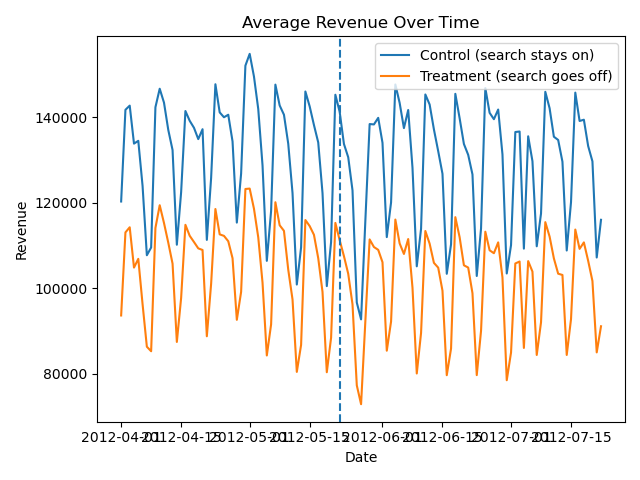
\includegraphics[width=0.85\textwidth]{../output/figures/figure_5_2.png}
\caption{Average revenue for treatment and control DMAs over time.
The dashed line marks May 22, 2012, when SEM was turned off
for the treatment group.}
\label{fig:revenue}
\end{figure}

Figure~\ref{fig:revenue} shows average revenue over time for treatment and control DMAs. The control group has consistently higher average revenue levels, reflecting the exclusion of the largest DMAs from treatment. Both groups display similar weekly oscillation patterns, suggesting comparable demand cycles across markets. At this scale, there is no dramatic visual divergence between the groups at the start of treatment, indicating that any effect is likely modest relative to overall revenue variation.

\begin{figure}[h]
\centering
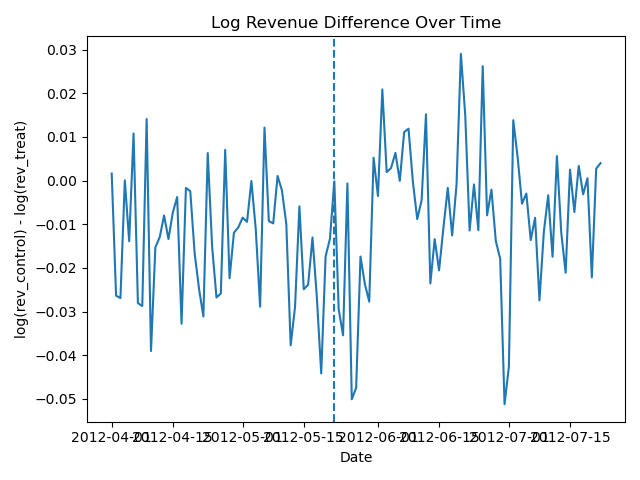
\includegraphics[width=0.85\textwidth]{../output/figures/figure_5_3.png}
\caption{Log-scale average revenue difference between control and treatment
groups over time. The gap appears to increase after May 22.}
\label{fig:logdiff}
\end{figure}

Figure~\ref{fig:logdiff} presents the log difference in average revenue between control and treatment groups over time. Before May 22, the log gap fluctuates around a relatively stable level, which is consistent with approximately parallel pre-treatment trends. After the intervention date, the gap appears to widen slightly, suggesting that treated markets may have experienced a relative decline in revenue. This visual pattern motivates estimating the treatment effect formally using a DID regression.


\section{Results}

\input{../output/tables/did_table.tex}

The DID estimate for the treatment interaction is $\hat{\gamma} = -0.0066$ in log points. Converting this to a proportional effect gives $\exp(-0.0066) = 0.9934$, which implies that treated DMAs experienced about a 0.66\% revenue decline when paid search was suspended.

However, statistical uncertainty is substantial relative to this point estimate. The 95\% confidence interval is $[-0.0175,\ 0.0043]$, which includes zero. Therefore, the null hypothesis of no effect cannot be rejected at the 5\% level. Economically, the estimate suggests at most a small negative impact, and the evidence is consistent with little to no meaningful revenue loss from stopping paid search for a strong brand like eBay. One interpretation is that many users who clicked paid ads would have reached eBay through unpaid channels anyway.

\section{Conclusion}
This replication finds that turning off paid search advertising led to a small and statistically insignificant change in eBay’s revenue. The difference-in-differences estimate closely mirrors the main finding reported by Blake et al. (2014): the effect of paid search for a well-known brand appears economically modest and not statistically distinguishable from zero at conventional levels. 

Several limitations should be acknowledged. The dataset used in this replication is scaled and shifted rather than raw revenue data, the treatment assignment excluded the largest DMAs and therefore was not fully randomized, and the analysis relies on a simple DID specification rather than a richer regression framework with additional controls. Despite these constraints, the core insight remains clear: conventional attribution metrics may substantially overstate the true incremental impact of paid search advertising. Careful causal identification is therefore critical when evaluating marketing return on investment.

\begin{thebibliography}{9}
\bibitem{blake2014}
Blake, T., C. Nosko, and S. Tadelis (2014).
``Consumer Heterogeneity and Paid Search Effectiveness: A Large-Scale Field Experiment.''
\textit{Econometrica}, 83(1): 155--174.

\bibitem{taddy2019}
Taddy, M. (2019).
\textit{Business Data Science}. McGraw-Hill, Chapter 5.
\end{thebibliography}

\end{document}
